\section{Empirical demonstration}

The resource was applied to nine bounded analytical objects. Mean Integration Accessibility was 63.9\% across six device--interface cases. Reproducibility Manifest Completeness was 54.2\% across three deployment objects. Physical Definition Completeness was 67.0\% across four resource cases, and Observability Coverage was 52.5\% across four execution or diagnostic cases. Two of three definitely classified partial-execution scenarios were preflight preventable, with an all-case sensitivity interval from 50.0\% to 75.0\%. A scheduling toy problem surfaced seven of eight incomplete requirement classes without resolving any to a scenario-specific value. Two of six bounded claims fully aligned test object, environment, acceptance rule, evidence, and claim scope. An AI-method discussion expanded from five opening context classes by ten core and seventeen broader reply-added classes. Five of twelve documentation-centered cases received a fully actionable public outcome.

The component metrics were recomputed with alternative partial-score weights from 0 through 1. Their central values depend on the conventional representation of partial evidence, confirming that they should be read as ordinal rubric summaries. Pairwise analysis among B2--B9 identified observability--recovery as the strongest relationship ($\phi=0.452$, lift $=2.353$). Leave-one-thread-out deletion retained the relationship above the pilot attention threshold in all 55 deletions. Observability--validation and interface accessibility--scheduling were also stable priorities. The validation--AI relationship remained exploratory because the AI stratum was small and threshold retention was limited.

These results demonstrate the resource's ability to preserve heterogeneous evidence, compute bounded summaries, expose sensitivity, and bind interpretations to source and denominator. They do not establish that the corpus represents the broader laboratory-automation field.

\begin{figure}[t]
  \centering
  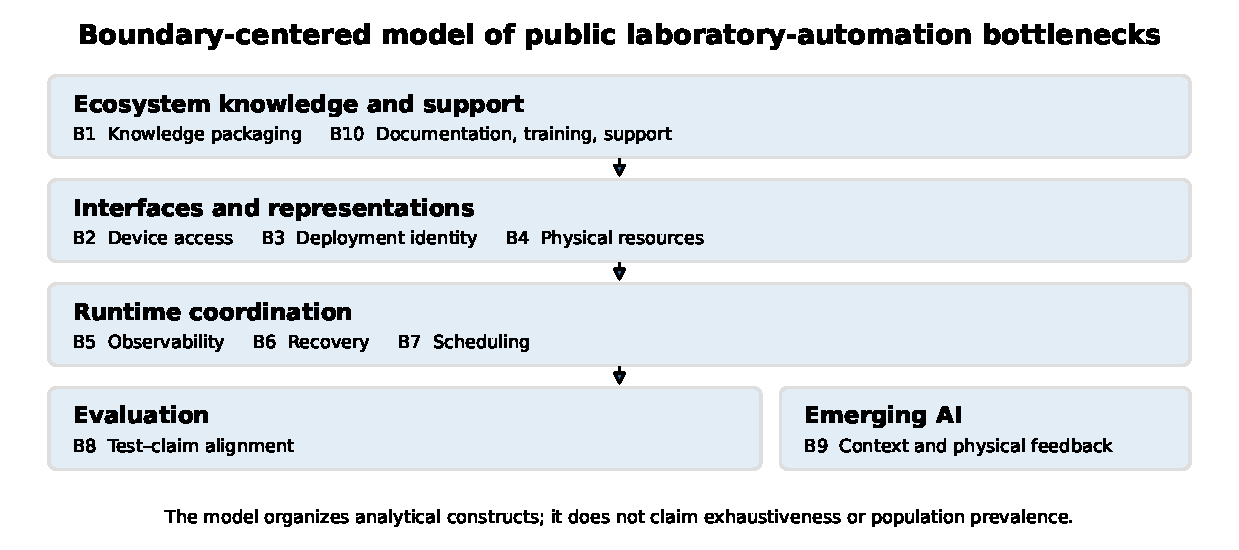
\includegraphics[width=\linewidth]{figures/conceptual_model.pdf}
  \caption{The released ten-construct model organizes ecosystem knowledge, interfaces and representations, runtime coordination, evaluation, and AI-specific context.}
\end{figure}

\begin{table}[t]
\centering
\caption{Bounded pilot metrics. Each row has a distinct unit and denominator.}
\label{tab:headline-metrics}
\begin{threeparttable}
\begin{tabularx}{\linewidth}{@{}L r l L@{}}
\toprule
Construct & Result & 95\% Wilson & Unit and denominator \\
\midrule
B2 Integration accessibility & 63.9\% & -- & 6 device--interface cases \\
B3 Deployment manifest & 54.2\% & -- & 3 deployment objects; 24 applicable cells \\
B4 Physical definitions & 67.0\% & -- & 4 resource definitions \\
B5 Observability & 52.5\% & -- & 4 execution/diagnostic cases \\
B6 Preflight preventability & 66.7\% & 20.8--93.9\% & 3 definite scenarios of 4 eligible \\
B7 Constraint discovery & 87.5\% & 52.9--97.8\% & 8 incomplete fields of 13 \\
B8 Fully aligned claims & 33.3\% & 9.7--70.0\% & 6 bounded claims \\
B9 Core context expansion & 2.0$\times$ & -- & 5 opening classes \\
B10 Actionable public outcome & 41.7\% & 19.3--68.0\% & 12 documentation cases \\
\bottomrule
\end{tabularx}
\begin{tablenotes}[flushleft]\footnotesize
\item Results demonstrate operationalization in selected cases. They do not estimate forum-wide or industry-wide rates.
\item Wilson intervals are descriptive uncertainty for the stated denominator, not population inference. A dash marks a row whose result is a mean of ordinal component scores or a ratio rather than a proportion, for which a binomial interval would be undefined.
\item Component means are taken over known cells only; unknown cells are excluded rather than scored as zero.
\end{tablenotes}
\end{threeparttable}
\end{table}

